\documentclass[aspectratio=169]{beamer}
\usetheme{Madrid}
\usepackage{graphicx}
\graphicspath{{images/}}
\setbeamertemplate{navigation symbols}{}
\setbeamertemplate{caption}{\raggedright\insertcaption\par}
\setbeamerfont{frametitle}{size=\large}

\title[SAE Dissection of SER]{Sparse-Autoencoder Dissection of\\Emotion Features in Frozen Speech Encoders}
\subtitle{From decodability to mechanism}
\author{Anonymous}
\date{}

\begin{document}

\begin{frame}\titlepage\end{frame}

\begin{frame}{The question}
Frozen speech encoders (HuBERT, WavLM, wav2vec2, w2v-BERT, MERT, Whisper) top SER benchmarks --- but they were trained for \textbf{ASR}, so they encode lots of \emph{text}.
\medskip
\begin{itemize}
  \item Probing tells us \textbf{where} emotion is readable. It cannot tell us:
  \item \emph{Which} features encode emotion?
  \item Is the signal \textbf{acoustic} (how it's said) or \textbf{lexical} (what's said)?
  \item Does the pattern hold across encoders and speakers?
\end{itemize}
\medskip
\textbf{Idea:} use \emph{Sparse Autoencoders} to go from \textbf{decodability} $\rightarrow$ \textbf{mechanism}.
\end{frame}

\begin{frame}{Method in one slide}
\begin{columns}
\begin{column}{0.58\textwidth}
\begin{itemize}
  \item Train a \textbf{TopK SAE} ($8\times$, $k{=}32$) on \textbf{per-frame} activations of each frozen encoder ($\sim$940k frames). FVU 0.07 (93\% variance), 4/8192 dead.
  \item Anchor on \textbf{CREMA-D}: 91 actors $\times$ 12 \emph{fixed} sentences $\times$ 6 emotions $\Rightarrow$ text is held constant, so any emotion signal is \emph{acoustic} (built-in control).
  \item \textbf{Confound-controlled emotion features:} keep a feature only if its firing tells us more about \emph{emotion} than about the \emph{sentence} (phonetics) or the \emph{speaker}.
\end{itemize}
\end{column}
\begin{column}{0.42\textwidth}
\centering
\footnotesize
394 naive features\\$\downarrow$ confound control\\\textbf{61 genuine} emotion features\\(median monosemanticity 0.59)\\[1ex]
dominated by \textbf{anger} \& \textbf{sadness};\\ fear/neutral $\to$ 0
\end{column}
\end{columns}
\medskip
\footnotesize Without confound control, $\sim$66\% of ``emotion'' features are really phonetic/speaker features --- the classic ``SAE rediscovers phonemes, not affect'' trap.
\end{frame}

\begin{frame}{Q1 --- Depth: decoding $\neq$ disentangling}
\begin{columns}
\begin{column}{0.5\textwidth}
\begin{itemize}
  \item Probe accuracy peaks \textbf{deep} (L10) and stays high.
  \item But clean monosemantic emotion features peak \textbf{early} (L7; monosemanticity L2).
  \item Deep layers keep \emph{decodability} but lose \emph{disentanglement} (24--47 feats).
\end{itemize}
\medskip
\textbf{Takeaway:} emotion is \emph{organised} into clean features earlier than where a probe reads it best.
\end{column}
\begin{column}{0.5\textwidth}
\centering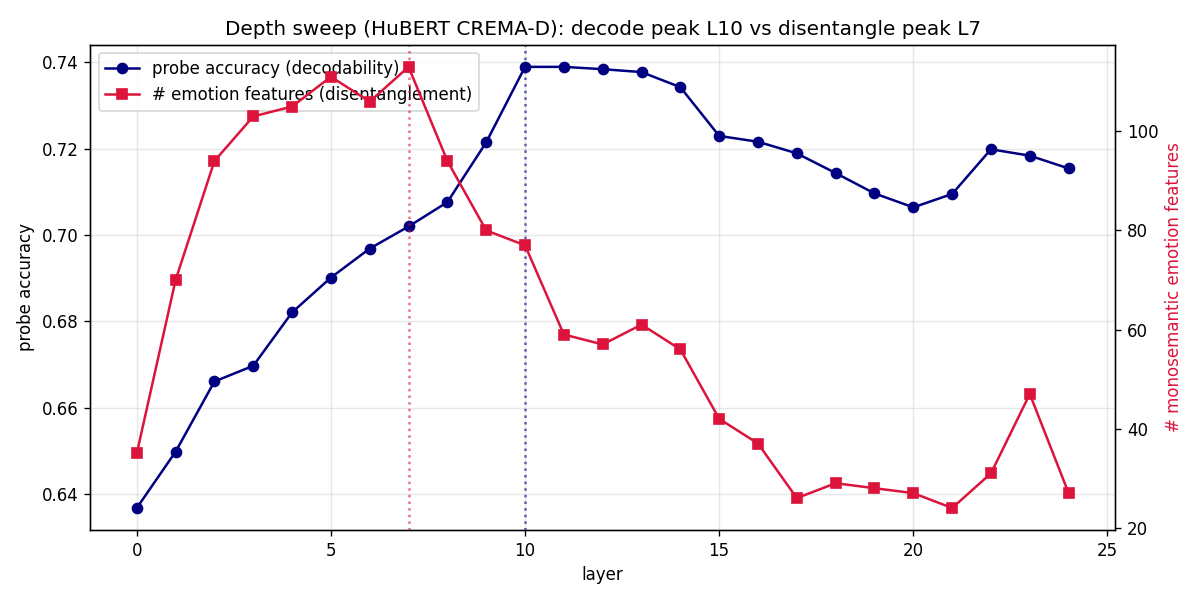
\includegraphics[width=\columnwidth]{fig_depth.png}
\end{column}
\end{columns}
\end{frame}

\begin{frame}{Q2 --- Across encoders \& speakers}
\begin{itemize}
  \item All six encoders carry emotion features (61--145 each), all anger/sadness-dominated.
  \item Cross-encoder feature overlap: \textbf{Whisper$\to$SSL 0.40 $\approx$ SSL$\to$SSL 0.39} --- on fixed-lexicon speech Whisper is \emph{not} special; its difference is about \emph{text}, not acoustics.
  \item \textbf{Speaker-invariant:} leave-speaker-out (91 actors) accuracy drop $\approx 0$; each feature fires for $\sim$95\% of its emotion's actors.
  \item $\Rightarrow$ the published MESD leave-one-speaker-out collapse ($\sim$0.30) is due to the \emph{speaker-entangled} features our control removes.
\end{itemize}
\end{frame}

\begin{frame}{Q3 --- The signal is acoustic, not lexical}
\begin{columns}
\begin{column}{0.5\textwidth}
\begin{itemize}
  \item Positive control: \textbf{60/61} features label \emph{acoustic} (eGeMAPS AUC 0.83 vs sentence 0.66).
  \item Causal \emph{sufficiency}: emotion decodes at \textbf{0.55} from acoustic features vs \textbf{0.43} lexical vs \textbf{0.42} random (full 0.73).
\end{itemize}
\medskip
\textbf{Takeaway:} what the probe exploits is paralinguistic delivery, not words.
\end{column}
\begin{column}{0.5\textwidth}
\centering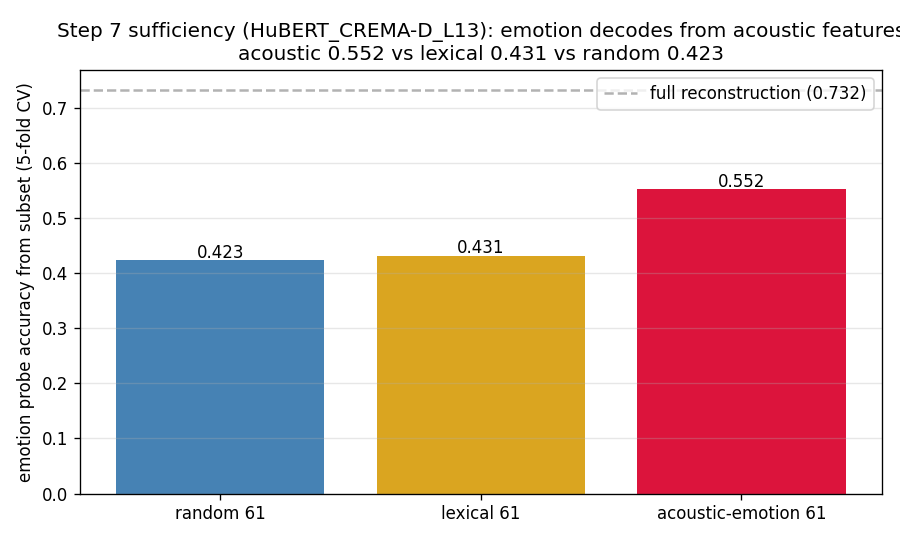
\includegraphics[width=\columnwidth]{fig_sufficiency.png}
\end{column}
\end{columns}
\end{frame}

\begin{frame}{Q4 --- EMIS: the lexical shortcut is a deep-layer thing}
\begin{columns}
\begin{column}{0.5\textwidth}
\begin{itemize}
  \item EMIS = synthetic speech where \emph{text} emotion $\neq$ \emph{voice} emotion.
  \item Train on congruent, test on incongruent; text-bias $=$ text$-$audio acc.
  \item Shortcut appears \textbf{only in deep layers} of ASR-SSL (HuBERT/WavLM/wav2vec2, $+0.7$--$0.9$).
  \item \textbf{Whisper stays audio-grounded at every layer} (L24 $-0.11$); MERT/w2v-BERT never take it.
  \item Reproduces the published text-bias --- and \emph{localizes} it to depth.
\end{itemize}
\end{column}
\begin{column}{0.5\textwidth}
\centering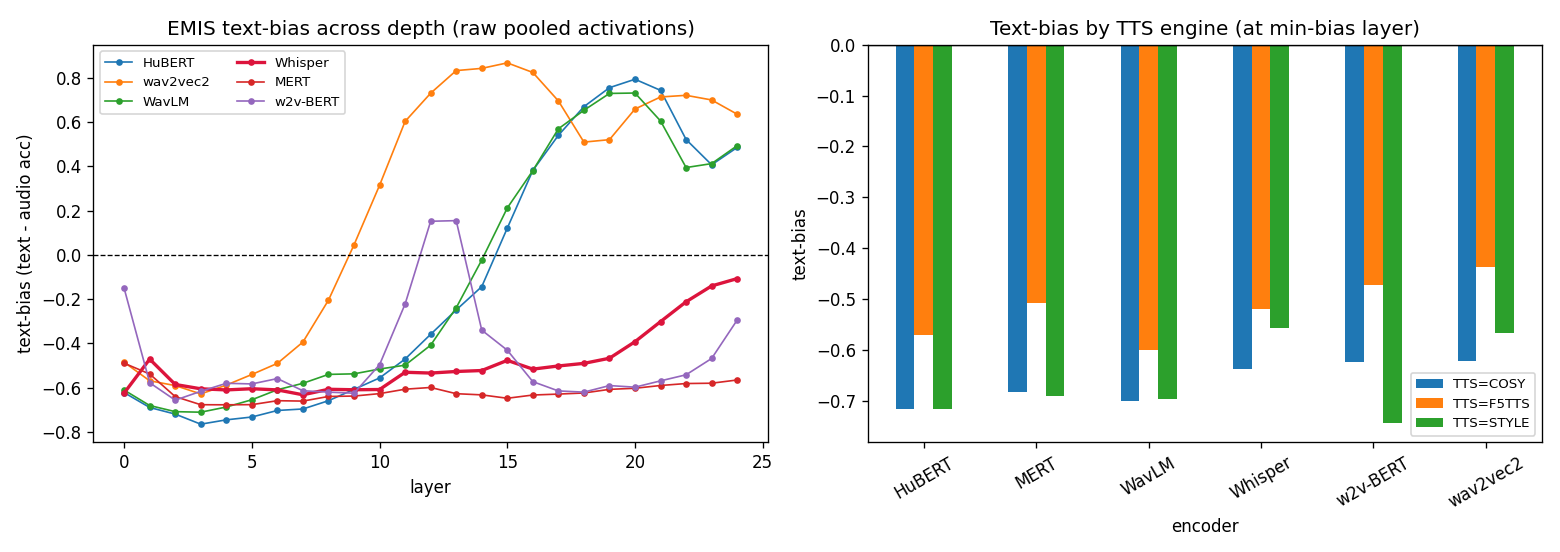
\includegraphics[width=\columnwidth]{fig_emis.png}
\end{column}
\end{columns}
\end{frame}

\begin{frame}{Where this sits in the literature}
\begin{itemize}
  \item \textbf{AudioSAE} (EACL 2026): same SAE recipe on 2 encoders, but emotion is just one probe task --- \emph{no} emotion-feature interpretation, confound control, factorial corpus, or acoustic/lexical split. Closest method neighbor.
  \item ASR-SAE works (Pluth'26; Mariotte'26): SAEs on speech, but find phonetic/lexical or singing features --- no affect, no depth sweep.
  \item Ma et al.\ '25: mechanistic Whisper-SER --- but via probing/CKA, \textbf{no SAEs}.
\end{itemize}
\medskip
\textbf{Un-scooped core:} confound-controlled SAE emotion features on a lexicon-controlled factorial corpus across 6 encoders $+$ decode$\neq$disentangle depth $+$ EMIS-shortcut-by-depth.
\end{frame}

\begin{frame}{Limitations \& future work}
\textbf{Limitations}
\begin{itemize}
  \item Necessity-ablation is near-null (signal distributed) --- we rely on sufficiency.
  \item SAE reconstruction must \emph{not} replace raw activations for the EMIS probe (it inverted Whisper).
  \item Cross-encoder/EMIS arms use one layer per encoder, not full 25-layer grids.
\end{itemize}
\textbf{Future work}
\begin{itemize}
  \item IEMOCAP real-transcript causal ablation (stub ready; needs transcripts).
  \item SpeechCraft cross-lingual feature overlap $\to$ explain EN$\leftrightarrow$ZH collapse.
  \item Feature \emph{steering}; dimensional V/A/D targets; full per-encoder layer grids.
\end{itemize}
\end{frame}

\begin{frame}{Takeaways}
\begin{enumerate}
  \item SAEs move SER analysis from \emph{decodability} to \emph{mechanism}; confound control is essential.
  \item \textbf{Decoding $\neq$ disentangling}: emotion organises early (L2--L7), decodes best deep (L10).
  \item Emotion features are \textbf{acoustic} and \textbf{speaker-invariant}, shared across all six encoders.
  \item The \textbf{lexical shortcut} is a deep-layer ASR-SSL phenomenon; \textbf{Whisper resists it everywhere}.
\end{enumerate}
\vfill
\footnotesize All code (\texttt{src/sae/}), data pointers, artifacts (\texttt{results/SAE/}) and the report are released on the \texttt{SAE} branch.
\end{frame}

\end{document}
